\section{Framework and Infrastructure}
\label{sec:infrastructure}


\begin{figure}
  \centering
  
\includegraphics[width=1.0\textwidth]{figs/framework.pdf}
  \caption{Framework of the AgentEvolver System.}
  \label{fig:infra_framework}
\end{figure}


\subsection{Training Framework}
\label{sec:framework}

This section introduces the training framework that turns the three mechanisms---\texttt{self-questioning}, \texttt{self-navigating}, and \texttt{self-attributing}---into an end-to-end, service-oriented system. The design emphasizes (i) a clear dataflow from environments to model updates, (ii) a hierarchical rollout stack tailored to agentic, multi-turn interaction, and (iii) algorithmic extensibility via modular, decoupled components.

\paragraph{Overall Architecture and Data Flow.}
As illustrated in Figure~\ref{fig:infra_framework}, a \emph{Master Orchestrator} drives a four-stage loop:
(A) \textbf{Task Synthesis}, (B) \textbf{Trajectory Rollout}, (C) \textbf{Experience Summarization}, and (D) \textbf{Sample Construction \& Model Optimization}.
First, \emph{Task Synthesis} is handled by a \emph{Task Manager}, which performs \textbf{self-questioning} by interacting with the environment to explore and automatically generate candidate training tasks.
\emph{Trajectory Rollout} then launches parallel executions of these tasks, where multiple rollout workers conduct multi-turn interactions between the model and the environment to generate diverse trajectories.
Next, \emph{Experience Summarization} is performed by the \textbf{Experience Manager}, which condenses historical trajectories into compact \emph{experience texts} (e.g., skills, tactics, or failure notes).
These summaries are indexed and retrieved during future rollouts to provide in-context guidance (ICL), enabling \texttt{self-navigating} rollouts that improve rollout quality and exploration efficiency.
Finally, \emph{Sample Construction \& Model Optimization} applies \texttt{self-attributing} to convert trajectories and intermediate states into training samples with fine-grained credit assignment (e.g., step-level attribution) and updates the policy parameters accordingly.


\paragraph{Hierarchical Rollout Execution For Agentic Multi-turn Interaction.}
To support complex multi-turn interactions at scale, the rollout process is organized into three hierarchical layers, as illustrated in Figure~\ref{fig:infra_framework}:
\begin{enumerate}
\item \textbf{Service Layer (bottom):} Comprising the \emph{Environment Server} and \emph{LLM Server}, this layer manages multiple independent environment or model workers.
Each worker handles a single environment step or model inference request and exposes standardized interfaces that can be accessed by rollout workers.
\item \textbf{Rollout Workers (middle):} The basic unit for sampling a trajectory.
Each worker interacts with the environment to initialize instances, execute actions, and collect observations, and with the model to assemble prompts and invoke the LLM in sequence, generating a complete trajectory for a given task.
\item \textbf{Rollout Manager / Master (top):} Oversees scheduling of multiple rollout workers, defines termination criteria, and coordinates curriculum strategies across workers.
\end{enumerate}
A key design principle is the \emph{decoupling of agent logic from runtime services}: the environment and LLM are provided as independent services, while the agent logic is encapsulated in a \emph{context manager} (described in Section \ref{sec:cmt}) that composes prompts from the current state.
This separation allows the same rollout infrastructure to host diverse agent workflows—such as ReAct policies, planner–executor schemes, or tool-using agents—without modification to the service layer.

\paragraph{Algorithmic Extensibility.}
The framework is designed to separate algorithmic logic from the underlying infrastructure, so that new methods can be introduced without altering the runtime services:
\begin{itemize}
\item \textbf{Task Manager.} Handles task generation and filtering.
Developers can freely switch between different task–synthesis modules and task–filtering strategies to explore alternative curricula or environment–specific goals.
\item \textbf{Rollout \& Context Manager.} Controls the agent’s multi-turn interaction logic.
By modifying the \emph{context manager}, developers can restructure the agentic flow—for example implementing ReAct, planner–executor, or other reasoning patterns—without changing the service layer.
\item \textbf{Experience Manager.} Summarizes past trajectories into concise experience texts and retrieves them during future rollouts.
Alternative summarization or retrieval mechanisms can be integrated to guide exploration and improve in-context learning.
\item \textbf{Training Pipeline.} Supports interchangeable sample-generation methods and model-optimization algorithms, such as different credit-assignment schemes, advantage estimators, or loss objectives.
\end{itemize}

These modules operate within a unified orchestration loop, allowing researchers to extend or replace any stage while maintaining a stable interface to the rest of the system.

\subsection{Context Manager}
\label{sec:context-manager}

\begin{figure}
  \centering
  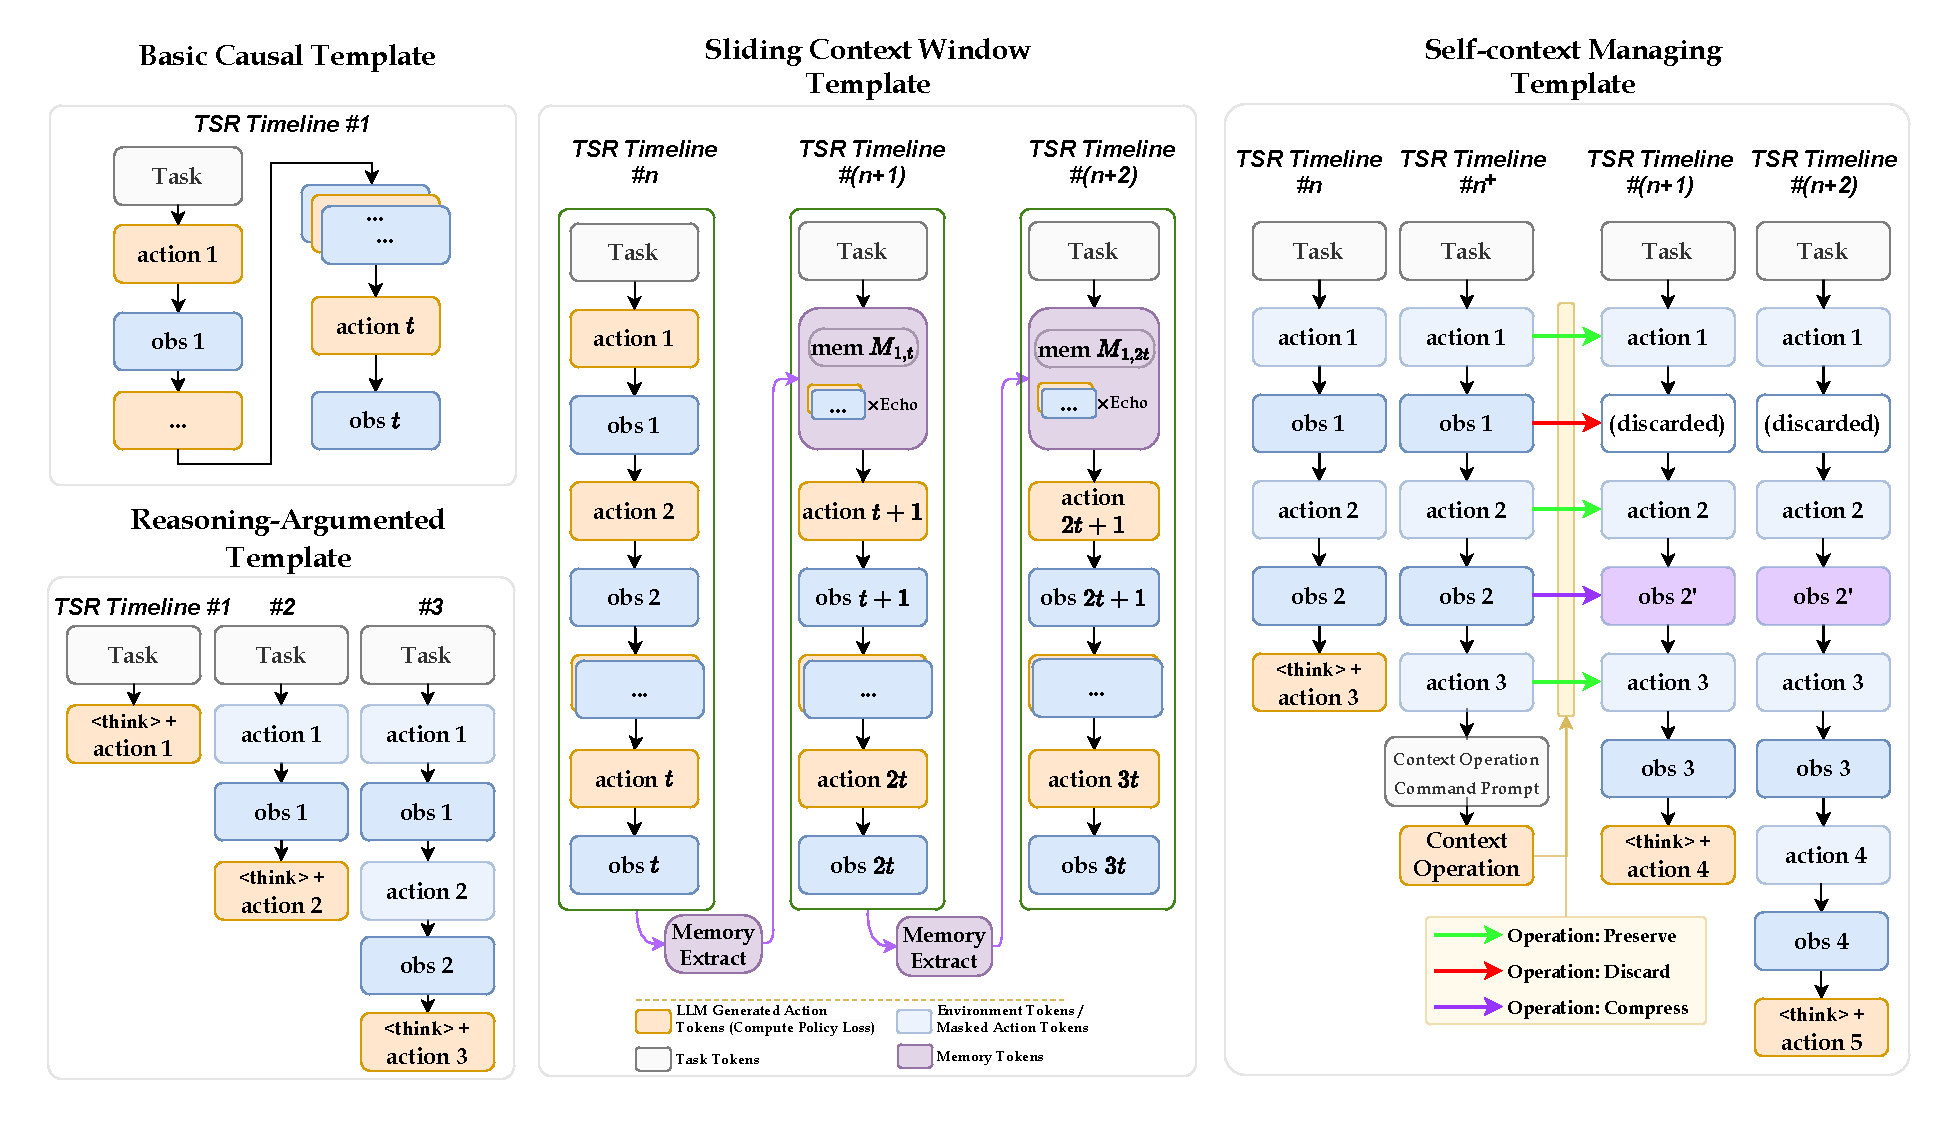
\includegraphics[width=1.0\textwidth]{figs/cmt_basic_four_4.drawio_new.pdf}
  \caption{The four fundamental context managing templates of AgentEvolver. Yellow blocks indicate LLM messages, blue blocks correspond to environment messages or messages masked from loss function, and purple blocks represent memory messages. The displayed timelines depict the anticipated outcomes after the Timeline Snapshot Recorder (TSR) completes the timeline merging process.}
  \label{fig:cmts}
\end{figure}


Long-horizon reinforcement learning with large language models (LLMs) requires not only reasoning and planning, but also dynamic management of historical context across multiple interactions. 
Existing paradigms exhibit a trade-off: the \emph{causal multi-step rollout} paradigm maintains strong temporal consistency but lacks flexibility~\citep{jin2025search}, while the \emph{step-independent multi-turn rollout} paradigm offers full editability at the cost of significant computational overhead~\citep{feng2025group}. 
To unify these two perspectives, AgentEvolver introduces a \textbf{Context Manager (CM)} that serves as the central infrastructure for controlling context evolution during agent–environment interactions.

The CM provides a consistent interface for both causal and non-causal interaction modes, enabling efficient, adaptive, and reasoning-aware rollouts. 
Its design aims to (1) maintain the computational efficiency of causal training, (2) allow selective modification of historical context when necessary, and (3) support agents that can eventually \emph{self-manage} their own context. 
To achieve this, CM introduces two fundamental data structures shared across all rollout paradigms.

\paragraph{Core Abstractions: Live Timeline and Snapshot Recorder.}
The Context Manager operates on two simple yet powerful primitives:
\begin{itemize}
    \item \textbf{Live Context Timeline (LCT)} — a mutable sequence representing the agent’s current working context during multi-turn interaction.
    \item \textbf{Timeline Snapshot Recorder (TSR)} — an immutable buffer that stores frozen snapshots of the LCT whenever the policy LLM generates an action.
\end{itemize}

The LCT acts as the agent’s short-term, editable memory, while the TSR maintains a verifiable, token-level record of the entire episode. 
After each rollout, the TSR automatically performs \emph{timeline merging}, removing redundant subsequences and aligning loss masks across overlapping segments. 
This dual-structure design allows CM to support both efficient causal rollouts and flexible reasoning-oriented rollouts within a unified framework.

\subsubsection{Rollout Paradigms and Context-Managing Templates}
\label{sec:cmt}

Built upon the LCT–TSR abstraction, the Context Manager defines a family of \textbf{Context-Managing Templates (CMTs)}. 
Each template specifies how the LCT evolves during interaction, thus representing a different balance between efficiency, reasoning capacity, and autonomy. 
The four fundamental templates are illustrated in Figure~\ref{fig:cmts}.

\paragraph{(i) Basic Causal Template — Efficient and Deterministic.}
The simplest template follows a strictly causal organization of messages. 
At the beginning of an episode, the initial task instruction is appended to the LCT. 
The agent then repeats the observe–act cycle until termination, after which only the final LCT snapshot is retained by the TSR.
This design ensures full temporal consistency and low computational cost, making it ideal for search-style RL training~\citep{jin2025search}. 
However, since messages cannot be edited or removed, memory consumption grows linearly with context length, and the lack of editability complicates reasoning-intensive behaviors.

\paragraph{(ii) Reasoning-Augmented Template — Structured Thinking Before Action.}
Reasoning before action has proven beneficial in complex decision-making tasks~\citep{guo2025deepseek}. 
The reasoning-augmented template trains agents to explicitly \emph{think before acting}. 
For models without pre-trained reasoning ability (e.g., Qwen2~\citep{team2024qwen2}), structured prompts encourage the model to generate \texttt{<think>} tokens before decisions, with additional rewards promoting high-quality reasoning. 
For models that already possess reasoning skills (e.g., Qwen3-14B~\citep{qwen2025technical}), the template enhances consistency and efficiency. 

\paragraph{(iii) Sliding Context Window Template — Scalable to Long Horizons.}
Long-horizon tasks often generate hundreds or thousands of interaction steps, exceeding the token capacity of typical LLMs. 
To address this, the sliding context window template treats the LCT as a moving window. 
When its size exceeds a predefined threshold, the Context Manager summarizes older content into a compressed \textit{memory message} and initializes a new timeline window for subsequent interactions. 
After timeline merging, only a minimal set of window snapshots remains. 
This approach preserves local causality while keeping GPU memory usage constant, achieving scalability to arbitrarily long episodes.

\paragraph{(iv) Self-Context Managing Template — Toward Autonomy.}
The previous templates rely on fixed rules for context updates. 
In contrast, the self-context managing template allows the agent to \emph{actively control} its own memory. 
When the LCT exceeds a token limit, the CM triggers a special \textit{context operation prompt}, asking the policy LLM to select for each message one of three operations:
\[
a_\text{context} \in \{\alpha_\text{keep}, \alpha_\text{remove}, \alpha_\text{compress}\},
\]
corresponding to preservation, deletion, and compression (via an external summarizing LLM).
This paradigm enables fine-grained control over the token budget and encourages the emergence of self-regulated information filtering behavior. 
It is particularly effective in environments that generate large amounts of uninformative text.

\paragraph{Discussion.}
All four templates share the same underlying LCT–TSR mechanism but differ in how they manipulate or delegate control over context evolution. 
Together, they form a spectrum from rigid causality to full autonomy: the Basic Causal Template maximizes efficiency, while the Self-Context Managing Template empowers agents to regulate their own memory dynamically. 
This unified view of context management provides a principled foundation for building scalable, reasoning-capable, and self-adaptive LLM agents.



\subsection{Environment Service: A Scalable and Gym-Compatible Execution Backend}\label{sec:env_service}

To support flexible and high-performance agent-environment interaction, we present an Environment Service that offers a scalable, service-oriented execution backend compatible with the OpenAI Gym interface. In contrast to traditional Gym environments that are tightly coupled with the training loop, our system decouples environment execution into an independent service, enabling remote, concurrent, and isolated environment instances on demand.

\textbf{Standardized Interface} \quad
We implement a minimal, Gym-compatible interface that defines core functionalities such as initialization, state retrieval, step-wise execution, evaluation, and lifecycle management. The interface is fully parameterizable, supporting dynamic runtime configuration of environment behavior. In addition to classical task environments, our design allows seamless integration with open-world tools and modular components such as Model Context Protocols (MCPs) and user-defined functions (UDFs), extending the range of supported scenarios. This unified interface ensures compatibility across diverse experimental settings while maintaining modularity and reusability.

\textbf{High-Concurrency Execution with Ray} \quad
To support large-scale concurrent training, each environment instance is executed as an isolated actor using Ray, a distributed computing framework. This approach provides efficient, lightweight isolation without relying on container-based sandboxing, significantly reducing overhead. Environment instances can be launched and terminated dynamically, enabling flexible scaling across CPU and GPU resources with support for both asynchronous and synchronous interaction modes.

\textbf{Lightweight Deployment and Integration} \quad
The Environment Service is designed for ease of deployment and minimal integration overhead. Preconfigured environments—including \textit{AppWorld} \citep{trivedi2024appworld}, \textit{BFCL} \citep{patil2025bfcl}, \textit{WebShop} \citep{yao2022webshop}, and \textit{Crafter} \citep{hafner2021benchmarking}—can be launched via Docker or installed via Python packages. Once deployed, the service exposes a unified HTTP interface for query submission and agent interaction, allowing training pipelines to operate without concerns over dependency conflicts or environment-specific installations.